\documentclass{article}
\usepackage[utf8]{inputenc}
\usepackage{geometry}
\usepackage{graphicx}
\usepackage{amsmath}
\usepackage{amsfonts}
\usepackage{amsthm}
\usepackage{amssymb}
\usepackage[most]{tcolorbox}
\usepackage{array}
\usepackage{latexsym}
\usepackage{alltt}
\usepackage{hyperref}
\usepackage{color, colortbl}
\usepackage{float}
\usepackage{pdfpages}
\usepackage{algpseudocode}
\usepackage{multicol}
\usepackage{multirow}
\usepackage{caption}
\usepackage{xparse}
\usepackage{setspace}
\usepackage{enumitem}
\usepackage{pdflscape}
% \usepackage{parskip}
\usepackage{blindtext}
\usepackage{forest}
\usepackage[newfloat]{minted}
\usepackage{booktabs}


\geometry
{
  a4paper,
  left=12mm,
  right=12mm,
  top=12mm,
  bottom=15mm,
}

% mybox
\newtcolorbox{mybox}[3][]
{
  colframe = #2!25,
  colback  = #2!10,
  coltitle = #2!20!black,  
  title    = {#3},
  #1,
}

\definecolor{bg}{rgb}{0.95,0.95,0.95}
\setminted
{
	mathescape=true,
	xleftmargin=\parindent,
	bgcolor=bg,
  escapeinside=@@
}

\SetupFloatingEnvironment{listing}{name=Code}

\usetikzlibrary{patterns,positioning,fit,arrows,calc,shapes.geometric,shapes.multipart,decorations.pathreplacing}


% New environments that use mybox
\newcounter{example}[section]
\newenvironment{example}[1]{\begin{mybox}[breakable]{green}{\refstepcounter{example}\textbf{Example \thesection.\theexample #1}}}{\end{mybox}}

\newcounter{definition}[section]
\newenvironment{definition}[1]{\refstepcounter{definition}\begin{mybox}[breakable]{blue}{\textbf{Definition \thesection.\thedefinition #1}}}{\end{mybox}}

\newcounter{theorem}[section]
\newenvironment{theorem}[1]{\begin{mybox}{red}{\refstepcounter{theorem}\textbf{Theorem \thesection.\thetheorem #1}}}{\end{mybox}}

\newenvironment{formula}[1]{\begin{mybox}{cyan}{\textbf{#1}}}{\end{mybox}}

% Changing maketitle
\makeatletter         
\renewcommand\maketitle{
{\raggedright % Note the extra {
\begin{center}
{\Large \bfseries \@title}\\[2ex] 
{\large \@author \ - \@date}\\[2ex]
\end{center}}} % Note the extra }
\makeatother

% \onehalfspacing % adjust spacing
\setlength{\parskip}{0.5\baselineskip}

% macros
\newcommand{\prob}[1]{\textbf{\textit{P}}\left\{#1\right\}}
\newcommand{\expc}[1]{\mathbf{E}\left(#1\right)}
\newcommand{\expcs}[1]{\mathbf{E}^2\left(#1\right)}
\newcommand{\var}[1]{\text{Var}\left( #1 \right)}
\newcommand{\ra}{\rightarrow}
\newcommand{\Ra}{\Rightarrow}

\def\colorfline#1{\noalign{\color{#1} \hrule height 1pt}}
\def\colorline#1{\cr \noalign{\color{#1} \hrule height 1pt \vskip-3em}}

\NewDocumentCommand{\dsum}{%
    e{^_}
}{%
  {% 
    \displaystyle\sum
    \IfValueT{#1}{^{#1}}
    \IfValueT{#2}{_{#2}}
  }
}%

% maketitle variables
\title{CENG 242 - Chapter 6: Data Abstraction (Encapsulation)}
\author{Burak Metehan Tunçel}
\date{May 2022}

\begin{document}

\maketitle

\begin{multicols*}{2}
\setlength{\columnsep}{1.5cm}
\setlength{\columnseprule}{0.2pt}

\section{Program Units, Packages and Encapsulation}
\label{sec:packages-encapsulation}

A \textit{\textbf{program unit}} is any named part of a program that can be designed and implemented more-or-less independently. A well-designed program unit has a \textit{single purpose}, and has a \textit{simple application program interface}. If well designed, a program unit is likely to be modifiable (capable of being changed without forcing major changes to other program units), and is potentially reusable (capable of being used in many programs).

The \textit{\textbf{application program interface}} (or \textit{\textbf{API}}) of a program unit is the minimum information that application programmers need to know in order to use the program unit successfully.

For instance, a procedure's API consists of its \textit{identifier}, \textit{formal parameters}, and \textit{result type if any}, together with a \textit{specification of its observable behavior}. The procedure's API does \textit{not} include the algorithm used in its definition.

In large-scale program construction, complexity grows, and reusability and abstraction become important. For example,
\begin{table}[H]
  \centering
  \begin{tabular}{lp{.6\linewidth}}
    \rowcolor{blue!10} 50 lines & no abstraction is essential, all in main() \\
    \rowcolor{blue!5} 500 lines & function/procedure abstraction sufficient\\
    \rowcolor{blue!10} 5,000 lines & function groups forming modules, modules are combined to form the application\\
    \rowcolor{blue!5} 500,000 lines & heavy abstraction and modularization, all parts designed for reuse (libraries, components etc)
\end{tabular}
\end{table}

Therefore, a programming language whose only program units are procedures (such as \texttt{C}) is suitable only for small-scale program construction. For large-scale program construction, the language should support large-scale program units such as \textit{packages}, \textit{abstract types}, and \textit{classes}.

\subsection{Packages}
\label{subsec:packages}

A \textit{\textbf{package}} is a group of several components declared for a common purpose. In other words, a group of declarations put into a single body.

These components may be \textit{types}, \textit{constants}, \textit{variables}, \textit{procedures}, or indeed \textit{any entities} that may be declared in the programming language.

\vspace*{\fill}
\columnbreak

\texttt{C} has indirect way of packaging per source file. \texttt{Python} defines modules per source file. \texttt{C++} has namespaces.
\begin{listing}[H]
\begin{minted}[]{cpp}
namespace Trig {
  const double pi=3.14159265358979;
  double sin(double x) { ... }
  double cos(double x) { ... }
  double tan(double x) { ... }
  double atan(double x) { ... }
  ...
};
\end{minted}
\caption{}
\label{code:code1}
\end{listing}
\noindent These functions can be used as 
  \mint{cpp}{Trig::sin(Trig::pi/2+x) + Trig::cos(x)}
\noindent In \texttt{C++}, (::) is \textit{Scope} operator. In this way, \textit{identifier overlap is avoided}. There is no name collisions in \mintinline{cpp}{List::insert(...)} and \mintinline{cpp}{Tree::insert(...)}.


\subsection{Encapsulation}
\label{subsec:encapsulation}

In order to keep its API simple, a package typically makes only \textit{some of its components visible} to the application code that uses the package; these components are said to be \textit{\textbf{public}}. \textit{Other components are visible only inside the package}; these
components are said to be \textit{\textbf{private}}, and serve only to support the implementation of the public components.

A package with private components hides information that is irrelevant to the application code. This technique for making a simple API is called \textit{\textbf{encapsulation}}.

The \textit{\textbf{package specification}} declares only the \textit{public components}, while the \textit{\textbf{package body}} declares any \textit{private components}.The package specification gives the package's interface, while the package body provides the implementation details.

Building an independent and self complete set of function and variable declarations is \underline{\textit{packaging}}. Restricting access to this set only via a set of interface
function and variables is \underline{\textit{hiding and encapsulation}}.

\begin{figure}[H]
  \centering
  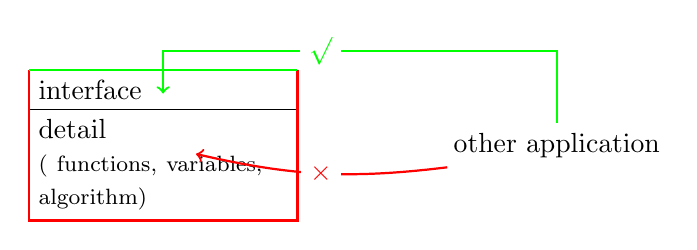
\begin{tikzpicture}[private/.style = {black,thick}, public/.style = {black,thick},
		pubcall/.style = {transparent}, pubtext/.style = {transparent},pricall/.style={transparent},
		pritext/.style={transparent} ]
    \tikzset{private/.style={red,thick}, public/.style = {green,thick}}
    \tikzset{pubcall/.style={green,draw,thick},pubtext/.style={green,fill=white}, pricall/.style={red,draw,thick},pritext/.style={red,fill=white}}
    \node [rectangle split, rectangle split parts=2, text width=9em,rectangle split draw splits=true] (box) {
      interface 
      \nodepart{two} 
      detail \\
      \footnotesize ( functions, variables, algorithm) 
    };
    \node [right of=box,xshift=4cm] (other) {other application};
    \draw (box.text split west) -- (box.text split east);
    \draw [private] (box.north west) -- (box.south west) -- (box.south east) -- (box.north east);
    \draw [public] (box.north west) -- (box.north east);
    \path [pubcall,->] (other) -- +(0,1.2) -| node [pubtext,pos=0.3] {$\surd$} (box.mid);
    \path [pricall,->,bend left=10] (other) to  node [pritext] {$\times$} ($(box.two) +(2cm,-2mm)$);
  \end{tikzpicture}
\end{figure}

\vspace*{\fill}
\columnbreak

\subsubsection*{Advantages of Encapsulation}
\label{subsubsec:adv-encap}

\begin{itemize}
  \item High volume details reduced to interface definitions (\textbf{Ease of development/maintenance})
  \item Many different applications use the same module via the same interface (\textbf{Code re-usability})
  \item Lego like development of code with building blocks (\textbf{Ease of
  development/maintenance}) 
  \item Even details change, applications do not change (as long as interface is kept same) (\textbf{Ease of development/maintenance})
  \item Module can be used in following projects (\textbf{Code re-usability})
\end{itemize}

\subsubsection*{Hiding}
\label{subsubsec:hiding}

A group of functions and variables hidden inside. The others are interface. Abstraction inside of a package:

\begin{table}[H]
  \begin{tabular}{|>{\tt}l|} \hline
    \color{gray}double taylorseries(double);  		\\
    double sin(double x);			\\
    double pi=3.14159265358979;		\\
    \color{gray}double randomseed;	\\
    double cos(double x);			\\
    \color{gray}double errorcorrect(double x); \\ \hline
  \end{tabular}
\end{table}
\begin{listing}[H]
\begin{minted}{Haskell}
{-- only sin, pi and cos are accessible --}
module Trig(sin,pi,cos) where
  taylorseries x = ... 
  sin x = ...
  pi=3.14159265358979
  randomseed= ...
  cos x = ...
  errorcorrect x = ...
\end{minted}
\caption{}
\label{code:code2}
\end{listing}



\section{Abstract Types}
\label{sec:abs-types}

Here is a summary of the difficulties that can arise in practice when a package has a public type component:
\begin{itemize}
  \item Application code can access the public type's representation directly. If we wish to change the representation (e.g., to make it more efficient), we have to modify not only the package but also any application code that accesses the representation directly. (Such code could be anywhere in the application program. Even if there turns out to be no such code, we have to read the whole program to be sure.)
  \item The public type's representation might have improper values that do not correspond to any values of the desired type. Even if the package's procedures are programmed correctly not to generate improper values, faulty application code might generate improper values.
  \item The public type's representation might be non-unique. A simple equality test might then yield the wrong result.
\end{itemize}

To avoid these problems we need an alternative way to define a new type. An \textit{\textbf{abstract type}} is a type whose identifier is public but whose representation is private. An abstract type must be equipped with a group of \textit{\textbf{operations}} to access its representation. The operations are typically procedures and constants. The values of the abstract type are defined to be just those values that can be generated by repeated use of the operations.

In other words, \textit{internals of the datatype is hidden and only interface functions provide the access}.
\begin{formula}{Example}
  rational numbers: 3/4 , 2/5, 19/3
\begin{listing}[H]
\begin{minted}[bgcolor={}]{haskell}
  data Rational = Rat (Integer, Integer)
  x = Rat (3,4)
  add (Rat(a,b)) (Rat(c,d)) = Rat (a*d+b*c,b*d)
\end{minted}
\end{listing}

  What about
\begin{itemize}
  \item[] Invalid value? \texttt{Rat (3,0)}
  \item[] Multiple representations of the same value?
    \texttt{Rat (2,4) = Rat (1,2) = Rat(3,6)}
\end{itemize}
Solution: avoid arbitrary values by the user.
\end{formula}

It does not matter whether an abstract type's representation is non-unique, because the representation is private. The key point is that only desired properties of the abstract type can actually be observed by application code using the operations with which the abstract type is equipped.

We can easily change an abstract type's representation: we need change only the package body and the private part of the package specification. We can be sure that we need not change the application code, since the latter cannot access the representation directly.

We can classify operations on an abstract type $T$ as follows.
\begin{itemize}
  \item A \textit{constructor} is an operation that computes a new value of type $T$, possibly using values of other types but not using an existing value of type $T$.
  \item A \textit{transformer} is an operation that computes a new value of type $T$, using an existing value of type $T$.
  \item An \textit{accessor} is an operation that computes a value of some other type, using an existing value of type $T$.
\end{itemize}
In general, we must equip each abstract type with \textit{at least one constructor}, \textit{at least one transformer}, and \textit{at least one accessor}. Between them, the constructors and transformers must be capable of generating all desired values of the abstract type.
\end{multicols*}

\begin{formula}{}

Main purpose of abstract data types is to use them transparently (as if they were built-in) without loosing data integrity.
\begin{listing}[H]
\begin{minted}[bgcolor={},escapeinside=\#\#]{haskell}
module Rational(#\color{red}{Rational,rat,add,subtract,multiply,divide}#) where
  data Rational = #\color{gray}{Rat}# (Integer,Integer)
  rat (x,y) = simplify (Rat(x,y))
  add (Rat(a,b)) (Rat(c,d)) = rat (a*d+b*c,b*d)  
  subtract(Rat(a,b)) (Rat(c,d)) = rat (a*d-b*c,b*d)  
  multiply(Rat(a,b)) (Rat(c,d)) = rat (a*c,b*d)
  divide (Rat(a,b)) (Rat(c,d)) = rat (a*d,b*c)
  #\color{gray}{gcd}# x y = if (x==0) then y
                            else if (y==0) then x
                            else if (x<y) then gcd x (y-x)
                            else gcd y (x-y)
  #\color{gray}{simplify}# (Rat(x,y)) = if y==0 then error "invalid value"
                                        else let a=gcd x y 
                                        in Rat(div x a, div y a)
\end{minted}
\end{listing}
\end{formula}

\begin{multicols*}{2}
\setlength{\columnsep}{1.5cm}
\setlength{\columnseprule}{0.2pt}


\section{Objects and Classes}
\label{sec:obj-class}

An \textit{\textbf{object}} is a group of variable components, equipped with a group of operations that access these variables.

\noindent Objects are/In objects;
\begin{itemize}
  \item Packages containing hidden variables and access is restricted to interface functions.
  \item Variables with state.
  \item Data integrity and abstraction provided by the interface functions.
  \item Entities in software can be modelled in terms of functions (server, customer record, document content, etc). Object oriented design.
\end{itemize}

\subsection{Classes}
\label{subsec:classes}

A \textit{\textbf{class}} is a set of similar objects. All the objects of a given class have the same variable components, and are equipped with the same operations.

Classes are supported by all the object-oriented languages including \texttt{C++} and \texttt{JAVA}. In object-oriented terminology, an object's variable components are variously called \textit{instance variables} or \textit{member variables}, and its operations are usually called \textit{constructors} and \textit{methods}.

A \textit{\textbf{constructor}} is an operation that creates (and typically initializes) a new object of the class. In both \texttt{C++} and \texttt{JAVA}, a constructor is always named after the class to which it belongs.

A \textit{\textbf{method}} is an operation that inspects and/or updates an existing object of the class.

\noindent Method call,
\mint{cpp}{O.M(E_1, @$\ldots$@, E_n)}
where
\begin{itemize}
  \item $O$ identifies the target object.
  \item $M$ is the name of method. If there is not method named $M$, it causes an error.
  \item $E_i$ are evaluated to yield the arguments.
\end{itemize}
Inside the method's body, \textbf{\texttt{this}} denotes the target object.

An \textit{object} is an \textit{\textbf{instance}} of the class that it belongs to (a counter type instead of a single counter). Classes have similar purposes to abstract data types.
\begin{listing}[H]

\begin{minted}{cpp}
class Counter {
private:   int counter;
public:    Counter() { counter=0; }
           int get() { return counter;}
           void increment() { counter++; }
} men,vehicles;
men.increment(); vehicles.increment();
men.get(); vehicles.get();
\end{minted}
\caption{C++ class declaration}
\label{code:code3}
\end{listing}

\begin{table}[H]
  \centering
  \textcolor{blue}{\large Abstract data type}\\
  \begin{tabular}{
    !{\color{red!70!black}\vrule width 1pt}p{7cm}
    !{\color{red!70!black}\vrule width 1pt}} \colorfline{green!70!black}
    interface {\footnotesize (constructor, functions)} \\ \hline \\
    detail {\footnotesize (\textcolor{red}{data type definition}, auxiliary functions)}  \colorline{red!70!black}
  \end{tabular}
\end{table}


\begin{table}[H]
  \centering
  \textcolor{blue}{\large Object}\\
  \begin{tabular}{
    !{\color{red!70!black}\vrule width 1pt}p{7cm}
    !{\color{red!70!black}\vrule width 1pt}} \colorfline{green!70!black}
    interface {\footnotesize (constructor, functions)}\\ \hline \\
    detail {\footnotesize (\textcolor{red}{variables}, auxiliary functions)}  \colorline{red!70!black}
  \end{tabular}
\end{table}

\begin{formula}{Purpose}
\begin{itemize}
  \item preserving data integrity, 
  \item abstraction, 
  \item re-usable codes.
\end{itemize}
\end{formula}


\subsection{Subclasses}
\label{subsec:subclasses}

Let $C$ denotes a class. A \textit{\textbf{subclass}} of $C$ is a set of objects that are similar to one another but richer than the objects of class $C$. An object of the subclass has all the variable components of an object of class $C$, but may have extra variable components. Likewise, an object of the subclass is equipped with all the methods of class $C$, but may be equipped with extra methods.

If $S$ is a subclass of $C$, we also say that $C$ is a \textit{\textbf{superclass}} of $S$.

A subclass is said to \textit{\textbf{inherit}} its superclass's variable components and methods. In certain circumstances, however, a subclass may \textit{\textbf{override}} some of its superclass's methods, by providing more specialized versions of these methods.

A \textit{private} component is visible only in its own class, while a \textit{public} component is visible everywhere. A \textit{\textbf{protected}} component is \textit{visible not only in its own class but also in any subclasses}. Protected status is therefore intermediate between private status and public status.


\section{Closure}
\label{sec:closure}

\textit{\textbf{Closure}} is an abstraction method using the saved environment state in a scope. When a function returns a \textit{local object} or \textit{function} as its result and language keeps the environment state along with the returned value, it becomes a \textit{closure}.

\begin{listing}[H]

\begin{minted}{py}
def newid():
  c = 0  # this is the hidden variable 
         # in the environment
  def incget():
    nonlocal c      #python 3, binds c above
    c += 1
    return c
  return incget

>>> a = newid()
>>> b = newid()
>>> a()
1
>>> b()
1
>>> b()
2
\end{minted}

\caption{}
\label{code:code4}
\end{listing}

\vspace*{\fill}
\columnbreak

Local variables of closures stay alive after call, as long as returned value is alive. \textbf{Closures} can be used for generating new functions as in higher order functions:
\begin{listing}[H]

\begin{minted}{py}
def mult(a):
  def nested(b):
    return a*b
  return nested # a different behaviour,
                # for each a value

twice = mult(2)
tentimes = mult(10)
a=twice(4)+tentimes(50)
\end{minted}

\caption{}
\label{code:code5}
\end{listing}

\noindent Also can be used for prototyping objects. \texttt{Javascript} example:
\begin{listing}[H]

\begin{minted}{js}
function counter() {
  var c = 0 // this is jailed in 
            //local environment, hidden
  var newobj = {} // create a new empty object
  newobj.incr = function () { c++; }
  newobj.get = function () { return c;}
  return newobj
}
a = counter()
b = counter()
a.incr()
a.get()
b.get()  
\end{minted}

\caption{}
\label{code:code6}
\end{listing}

\vspace*{\fill}
\columnbreak

\texttt{C++} 2011 implements closures in lambda expressions by adding a set of captured variables within [ ]. This copy or get reference of auto variables in the environment in an object.

However \texttt{C++} closures do not extend lifetime of captured variables. After exit, the behaviour is undetermined.

\mintinline[bgcolor={}]{cpp}{[a, &b] (int x) { return a+x+b;}} captures $a$ and $b$ from current environment, $a$ is by copy, $b$ by reference.
\begin{listing}[H]

\begin{minted}{cpp}
std::function<int(int)>  multiply(int a) {
  // capture by value
  return [&] (int b) { return a*b;};
};
std::function<int()> cid() {
  int c = 0;
  // capture by copy
  return [=] () mutable { return ++c; };
};
int main() {
  std::function<int(int)> twice = multiply(2);
  std::function<int(int)> three = multiply(3);

  cout << twice(12) << ' ' << three(34) << endl;

  auto c1 = cid();
  auto c2 = cid();

  cout << c1() << ' ' << c2() << endl;
  c1(); c1(); c1();
  cout << c1() << ' ' << c2() << endl;
  return 0;
}
\end{minted}

\caption{}
\label{code:code7}
\end{listing}


\end{multicols*}

\end{document}
